
%----------------------------------------------------------------------------------------
%	PACKAGES AND OTHER DOCUMENT CONFIGURATIONS
%----------------------------------------------------------------------------------------

\documentclass[11pt,fleqn,oneside]{book} % Default font size and left-justified equations

\usepackage[top=3cm,bottom=3cm,left=3.2cm,right=3.2cm,headsep=10pt,letterpaper]{geometry} % Page margins

\usepackage{array}
\usepackage{listings}
\usepackage{url}
\usepackage{amsmath}
\usepackage[usenames, dvipsnames]{color}
\usepackage{xcolor} % Required for specifying colors by name
\usepackage{forest}
\definecolor{folderbg}{RGB}{124,166,198}
\definecolor{folderborder}{RGB}{110,144,169}

\def\Size{4pt}
\tikzset{
  folder/.pic={
    \filldraw[draw=folderborder,top color=folderbg!50,bottom color=folderbg]
      (-1.05*\Size,0.2\Size+5pt) rectangle ++(.75*\Size,-0.2\Size-5pt);  
    \filldraw[draw=folderborder,top color=folderbg!50,bottom color=folderbg]
      (-1.15*\Size,-\Size) rectangle (1.15*\Size,\Size);
  }
}
\definecolor{ocre}{RGB}{52,177,201} % Define the orange color used for highlighting throughout the book
\usepackage{multicol}
\setlength{\columnsep}{1cm}
% Font Settings
\usepackage{avant} % Use the Avantgarde font for headings
%\usepackage{times} % Use the Times font for headings
\usepackage{mathptmx} % Use the Adobe Times Roman as the default text font together with math symbols from the Sym­bol, Chancery and Computer Modern fonts

\usepackage{microtype} % Slightly tweak font spacing for aesthetics
\usepackage[utf8]{inputenc} % Required for including letters with accents
\usepackage[T1]{fontenc} % Use 8-bit encoding that has 256 glyphs

% Bibliography
\usepackage[style=alphabetic,sorting=nyt,sortcites=true,autopunct=true,babel=hyphen,hyperref=true,abbreviate=false,backref=true,backend=biber]{biblatex}
\addbibresource{references.bib} % BibTeX bibliography file
\defbibheading{bibempty}{}

%----------------------------------------------------------------------------------------
%	VARIOUS REQUIRED PACKAGES
%----------------------------------------------------------------------------------------

\usepackage{titlesec} % Allows customization of titles

\usepackage{graphicx} % Required for including pictures
\graphicspath{{Pictures/}} % Specifies the directory where pictures are stored

\usepackage{lipsum} % Inserts dummy text

\usepackage{tikz} % Required for drawing custom shapes

\usepackage[english]{babel} % English language/hyphenation

\usepackage{enumitem} % Customize lists
\setlist{nolistsep} % Reduce spacing between bullet points and numbered lists

\usepackage{booktabs} % Required for nicer horizontal rules in tables

\usepackage{eso-pic} % Required for specifying an image background in the title page

%----------------------------------------------------------------------------------------
%	MAIN TABLE OF CONTENTS
%----------------------------------------------------------------------------------------

\usepackage{titletoc} % Required for manipulating the table of contents

\contentsmargin{0cm} % Removes the default margin
% Chapter text styling
\titlecontents{chapter}[1.25cm] % Indentation
{\addvspace{15pt}\large\sffamily\bfseries} % Spacing and font options for chapters
{\color{ocre!60}\contentslabel[\Large\thecontentslabel]{1.25cm}\color{ocre}} % Chapter number
{}  
{\color{ocre!60}\normalsize\sffamily\bfseries\;\titlerule*[.5pc]{.}\;\thecontentspage} % Page number
% Section text styling
\titlecontents{section}[1.25cm] % Indentation
{\addvspace{5pt}\sffamily\bfseries} % Spacing and font options for sections
{\contentslabel[\thecontentslabel]{1.25cm}} % Section number
{}
{\sffamily\hfill\color{black}\thecontentspage} % Page number
[]
% Subsection text styling
\titlecontents{subsection}[1.25cm] % Indentation
{\addvspace{1pt}\sffamily\small} % Spacing and font options for subsections
{\contentslabel[\thecontentslabel]{1.25cm}} % Subsection number
{}
{\sffamily\;\titlerule*[.5pc]{.}\;\thecontentspage} % Page number
[] 

%----------------------------------------------------------------------------------------
%	MINI TABLE OF CONTENTS IN CHAPTER HEADS
%----------------------------------------------------------------------------------------

% Section text styling
\titlecontents{lsection}[0em] % Indendating
{\footnotesize\sffamily} % Font settings
{}
{}
{}

% Subsection text styling
\titlecontents{lsubsection}[.5em] % Indentation
{\normalfont\footnotesize\sffamily} % Font settings
{}
{}
{}
 
%----------------------------------------------------------------------------------------
%	PAGE HEADERS
%----------------------------------------------------------------------------------------

\usepackage{fancyhdr} % Required for header and footer configuration

\pagestyle{fancy}
\renewcommand{\chaptermark}[1]{\markboth{\sffamily\normalsize\bfseries\chaptername\ \thechapter.\ #1}{}} % Chapter text font settings
\renewcommand{\sectionmark}[1]{\markright{\sffamily\normalsize\thesection\hspace{5pt}#1}{}} % Section text font settings
\fancyhf{} \fancyhead[LE,RO]{\sffamily\normalsize\thepage} % Font setting for the page number in the header
\fancyhead[LO]{\rightmark} % Print the nearest section name on the left side of odd pages
\fancyhead[RE]{\leftmark} % Print the current chapter name on the right side of even pages
\renewcommand{\headrulewidth}{0.5pt} % Width of the rule under the header
\addtolength{\headheight}{2.5pt} % Increase the spacing around the header slightly
\renewcommand{\footrulewidth}{0pt} % Removes the rule in the footer
\fancypagestyle{plain}{\fancyhead{}\renewcommand{\headrulewidth}{0pt}} % Style for when a plain pagestyle is specified

% Removes the header from odd empty pages at the end of chapters
\makeatletter
\renewcommand{\cleardoublepage}{
\clearpage\ifodd\c@page\else
\hbox{}
\vspace*{\fill}
\thispagestyle{empty}
\newpage
\fi}

%----------------------------------------------------------------------------------------
%	THEOREM STYLES
%----------------------------------------------------------------------------------------

\usepackage{amsmath,amsfonts,amssymb,amsthm} % For math equations, theorems, symbols, etc

\newcommand{\intoo}[2]{\mathopen{]}#1\,;#2\mathclose{[}}
\newcommand{\ud}{\mathop{\mathrm{{}d}}\mathopen{}}
\newcommand{\intff}[2]{\mathopen{[}#1\,;#2\mathclose{]}}
\newtheorem{notation}{Notation}[chapter]

%%%%%%%%%%%%%%%%%%%%%%%%%%%%%%%%%%%%%%%%%%%%%%%%%%%%%%%%%%%%%%%%%%%%%%%%%%%
%%%%%%%%%%%%%%%%%%%% dedicated to boxed/framed environements %%%%%%%%%%%%%%
%%%%%%%%%%%%%%%%%%%%%%%%%%%%%%%%%%%%%%%%%%%%%%%%%%%%%%%%%%%%%%%%%%%%%%%%%%%
\newtheoremstyle{ocrenumbox}% % Theorem style name
{0pt}% Space above
{0pt}% Space below
{\normalfont}% % Body font
{}% Indent amount
{\small\bf\sffamily\color{ocre}}% % Theorem head font
{\;}% Punctuation after theorem head
{0.25em}% Space after theorem head
{\small\sffamily\color{ocre}\thmname{#1}\nobreakspace\thmnumber{\@ifnotempty{#1}{}\@upn{#2}}% Theorem text (e.g. Theorem 2.1)
\thmnote{\nobreakspace\the\thm@notefont\sffamily\bfseries\color{black}---\nobreakspace#3.}} % Optional theorem note
\renewcommand{\qedsymbol}{$\blacksquare$}% Optional qed square

\newtheoremstyle{blacknumex}% Theorem style name
{5pt}% Space above
{5pt}% Space below
{\normalfont}% Body font
{} % Indent amount
{\small\bf\sffamily}% Theorem head font
{\;}% Punctuation after theorem head
{0.25em}% Space after theorem head
{\small\sffamily{\tiny\ensuremath{\blacksquare}}\nobreakspace\thmname{#1}\nobreakspace\thmnumber{\@ifnotempty{#1}{}\@upn{#2}}% Theorem text (e.g. Theorem 2.1)
\thmnote{\nobreakspace\the\thm@notefont\sffamily\bfseries---\nobreakspace#3.}}% Optional theorem note

\newtheoremstyle{blacknumbox} % Theorem style name
{0pt}% Space above
{0pt}% Space below
{\normalfont}% Body font
{}% Indent amount
{\small\bf\sffamily}% Theorem head font
{\;}% Punctuation after theorem head
{0.25em}% Space after theorem head
{\small\sffamily\thmname{#1}\nobreakspace\thmnumber{\@ifnotempty{#1}{}\@upn{#2}}% Theorem text (e.g. Theorem 2.1)
\thmnote{\nobreakspace\the\thm@notefont\sffamily\bfseries---\nobreakspace#3.}}% Optional theorem note

%%%%%%%%%%%%%%%%%%%%%%%%%%%%%%%%%%%%%%%%%%%%%%%%%%%%%%%%%%%%%%%%%%%%%%%%%%%
%%%%%%%%%%%%% dedicated to non-boxed/non-framed environements %%%%%%%%%%%%%
%%%%%%%%%%%%%%%%%%%%%%%%%%%%%%%%%%%%%%%%%%%%%%%%%%%%%%%%%%%%%%%%%%%%%%%%%%%
\newtheoremstyle{ocrenum}% % Theorem style name
{5pt}% Space above
{5pt}% Space below
{\normalfont}% % Body font
{}% Indent amount
{\small\bf\sffamily\color{ocre}}% % Theorem head font
{\;}% Punctuation after theorem head
{0.25em}% Space after theorem head
{\small\sffamily\color{ocre}\thmname{#1}\nobreakspace\thmnumber{\@ifnotempty{#1}{}\@upn{#2}}% Theorem text (e.g. Theorem 2.1)
\thmnote{\nobreakspace\the\thm@notefont\sffamily\bfseries\color{black}---\nobreakspace#3.}} % Optional theorem note
\renewcommand{\qedsymbol}{$\blacksquare$}% Optional qed square
\makeatother

% Defines the theorem text style for each type of theorem to one of the three styles above
\newcounter{dummy} 
\numberwithin{dummy}{section}
\theoremstyle{ocrenumbox}
\newtheorem{theoremeT}[dummy]{Theorem}
\newtheorem{problem}{Problem}[chapter]
\newtheorem{exerciseT}{Exercise}[chapter]
\theoremstyle{blacknumex}
\newtheorem{exampleT}{Example}[chapter]
\theoremstyle{blacknumbox}
\newtheorem{vocabulary}{Vocabulary}[chapter]
\newtheorem{definitionT}{Definition}[section]
\newtheorem{corollaryT}[dummy]{Corollary}
\theoremstyle{ocrenum}
\newtheorem{proposition}[dummy]{Proposition}

%----------------------------------------------------------------------------------------
%	DEFINITION OF COLORED BOXES
%----------------------------------------------------------------------------------------

\RequirePackage[framemethod=default]{mdframed} % Required for creating the theorem, definition, exercise and corollary boxes

% Theorem box
\newmdenv[skipabove=7pt,
skipbelow=7pt,
backgroundcolor=black!5,
linecolor=ocre,
innerleftmargin=5pt,
innerrightmargin=5pt,
innertopmargin=5pt,
leftmargin=0cm,
rightmargin=0cm,
innerbottommargin=5pt]{tBox}

% Exercise box	  
\newmdenv[skipabove=7pt,
skipbelow=7pt,
rightline=false,
leftline=true,
topline=false,
bottomline=false,
backgroundcolor=ocre!10,
linecolor=ocre,
innerleftmargin=5pt,
innerrightmargin=5pt,
innertopmargin=5pt,
innerbottommargin=5pt,
leftmargin=0cm,
rightmargin=0cm,
linewidth=4pt]{eBox}	

% Definition box
\newmdenv[skipabove=7pt,
skipbelow=7pt,
rightline=false,
leftline=true,
topline=false,
bottomline=false,
linecolor=ocre,
innerleftmargin=5pt,
innerrightmargin=5pt,
innertopmargin=0pt,
leftmargin=0cm,
rightmargin=0cm,
linewidth=4pt,
innerbottommargin=0pt]{dBox}	

% Corollary box
\newmdenv[skipabove=7pt,
skipbelow=7pt,
rightline=false,
leftline=true,
topline=false,
bottomline=false,
linecolor=gray,
backgroundcolor=black!5,
innerleftmargin=5pt,
innerrightmargin=5pt,
innertopmargin=5pt,
leftmargin=0cm,
rightmargin=0cm,
linewidth=4pt,
innerbottommargin=5pt]{cBox}

% Creates an environment for each type of theorem and assigns it a theorem text style from the "Theorem Styles" section above and a colored box from above
\newenvironment{theorem}{\begin{tBox}\begin{theoremeT}}{\end{theoremeT}\end{tBox}}
\newenvironment{exercise}{\begin{eBox}\begin{exerciseT}}{\hfill{\color{ocre}\tiny\ensuremath{\blacksquare}}\end{exerciseT}\end{eBox}}				  
\newenvironment{definition}{\begin{dBox}\begin{definitionT}}{\end{definitionT}\end{dBox}}	
\newenvironment{example}{\begin{exampleT}}{\hfill{\tiny\ensuremath{\blacksquare}}\end{exampleT}}		
\newenvironment{corollary}{\begin{cBox}\begin{corollaryT}}{\end{corollaryT}\end{cBox}}	

%----------------------------------------------------------------------------------------
%	REMARK ENVIRONMENT
%----------------------------------------------------------------------------------------

\newenvironment{remark}{\par\vspace{10pt}\small % Vertical white space above the remark and smaller font size
\begin{list}{}{
\leftmargin=35pt % Indentation on the left
\rightmargin=25pt}\item\ignorespaces % Indentation on the right
\makebox[-2.5pt]{\begin{tikzpicture}[overlay]
\node[draw=ocre!60,line width=1pt,circle,fill=ocre!25,font=\sffamily\bfseries,inner sep=2pt,outer sep=0pt] at (-15pt,0pt){\textcolor{ocre}{R}};\end{tikzpicture}} % Orange R in a circle
\advance\baselineskip -1pt}{\end{list}\vskip5pt} % Tighter line spacing and white space after remark

%----------------------------------------------------------------------------------------
%	SECTION NUMBERING IN THE MARGIN
%----------------------------------------------------------------------------------------

\makeatletter
\renewcommand{\@seccntformat}[1]{\llap{\textcolor{ocre}{\csname the#1\endcsname}\hspace{1em}}}                    
\renewcommand{\section}{\@startsection{section}{1}{\z@}
{-4ex \@plus -1ex \@minus -.4ex}
{1ex \@plus.2ex }
{\normalfont\large\sffamily\bfseries}}
\renewcommand{\subsection}{\@startsection {subsection}{2}{\z@}
{-3ex \@plus -0.1ex \@minus -.4ex}
{0.5ex \@plus.2ex }
{\normalfont\sffamily\bfseries}}
\renewcommand{\subsubsection}{\@startsection {subsubsection}{3}{\z@}
{-2ex \@plus -0.1ex \@minus -.2ex}
{.2ex \@plus.2ex }
{\normalfont\small\sffamily\bfseries}}                        
\renewcommand\paragraph{\@startsection{paragraph}{4}{\z@}
{-2ex \@plus-.2ex \@minus .2ex}
{.1ex}
{\normalfont\small\sffamily\bfseries}}

%----------------------------------------------------------------------------------------
%	HYPERLINKS IN THE DOCUMENTS
%----------------------------------------------------------------------------------------

% For an unclear reason, the package should be loaded now and not later
\usepackage{hyperref}
\hypersetup{hidelinks,backref=true,pagebackref=true,hyperindex=true,colorlinks=false,breaklinks=true,urlcolor= ocre,bookmarks=true,bookmarksopen=false,pdftitle={Title},pdfauthor={Author}}

%----------------------------------------------------------------------------------------
%	CHAPTER HEADINGS
%----------------------------------------------------------------------------------------

% The set-up below should be (sadly) manually adapted to the overall margin page septup controlled by the geometry package loaded in the main.tex document. It is possible to implement below the dimensions used in the goemetry package (top,bottom,left,right)... TO BE DONE

\newcommand{\thechapterimage}{}
\newcommand{\chapterimage}[1]{\renewcommand{\thechapterimage}{#1}}

% Numbered chapters with mini tableofcontents
\def\thechapter{\arabic{chapter}}
\def\@makechapterhead#1{
\thispagestyle{empty}
{\centering \normalfont\sffamily
\ifnum \c@secnumdepth >\m@ne
\if@mainmatter
\startcontents
\begin{tikzpicture}[remember picture,overlay]
\node at (current page.north west)
{\begin{tikzpicture}[remember picture,overlay]
\node[anchor=north west,inner sep=0pt] at (0,0) {\includegraphics[width=\paperwidth]{\thechapterimage}};
%%%%%%%%%%%%%%%%%%%%%%%%%%%%%%%%%%%%%%%%%%%%%%%%%%%%%%%%%%%%%%%%%%%%%%%%%%%%%%%%%%%%%
% Commenting the 3 lines below removes the small contents box in the chapter heading
%\fill[color=ocre!10!white,opacity=.6] (1cm,0) rectangle (8cm,-7cm);
%\node[anchor=north west] at (1.1cm,.35cm) {\parbox[t][8cm][t]{6.5cm}{\huge\bfseries\flushleft \printcontents{l}{1}{\setcounter{tocdepth}{2}}}};
\draw[anchor=west] (5cm,-9cm) node [rounded corners=20pt,fill=ocre!10!white,text opacity=1,draw=ocre,draw opacity=1,line width=1.5pt,fill opacity=.6,inner sep=12pt]{\huge\sffamily\bfseries\textcolor{black}{\thechapter. #1\strut\makebox[22cm]{}}};
%%%%%%%%%%%%%%%%%%%%%%%%%%%%%%%%%%%%%%%%%%%%%%%%%%%%%%%%%%%%%%%%%%%%%%%%%%%%%%%%%%%%%
\end{tikzpicture}};
\end{tikzpicture}}
\par\vspace*{230\p@}
\fi
\fi}

% Unnumbered chapters without mini tableofcontents (could be added though) 
\def\@makeschapterhead#1{
\thispagestyle{empty}
{\centering \normalfont\sffamily
\ifnum \c@secnumdepth >\m@ne
\if@mainmatter
\begin{tikzpicture}[remember picture,overlay]
\node at (current page.north west)
{\begin{tikzpicture}[remember picture,overlay]
\node[anchor=north west,inner sep=0pt] at (0,0) {\includegraphics[width=\paperwidth]{\thechapterimage}};
\draw[anchor=west] (5cm,-9cm) node [rounded corners=20pt,fill=ocre!10!white,fill opacity=.6,inner sep=12pt,text opacity=1,draw=ocre,draw opacity=1,line width=1.5pt]{\huge\sffamily\bfseries\textcolor{black}{#1\strut\makebox[22cm]{}}};
\end{tikzpicture}};
\end{tikzpicture}}
\par\vspace*{230\p@}
\fi
\fi
}
\makeatother % Insert the commands.tex file which contains the majority of the structure behind the template

\let\cleardoublepage\clearpage
\lstset { %
    language=C++,
    backgroundcolor=\color{black!5}, % set backgroundcolor
    basicstyle=\footnotesize,% basic font setting
}

\lstdefinestyle{customc}{
  belowcaptionskip=1\baselineskip,
  breaklines=true,
  frame=L,
  xleftmargin=\parindent,
  language=C,
  showstringspaces=false,
  basicstyle=\footnotesize\ttfamily,
  keywordstyle=\bfseries\color{green!40!black},
  commentstyle=\itshape\color{purple!40!black},
  identifierstyle=\color{blue},
  stringstyle=\color{orange},
}

\lstset{escapechar=@,style=customc}

\begin{document}

%----------------------------------------------------------------------------------------
%	TITLE PAGE
%----------------------------------------------------------------------------------------

\begingroup
\thispagestyle{empty}
\AddToShipoutPicture*{\put(0,0){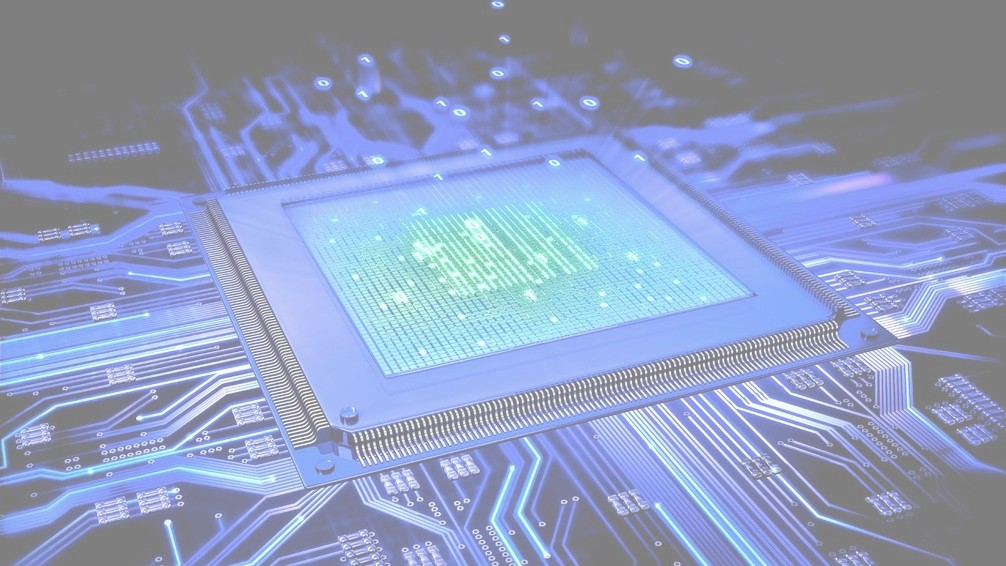
\includegraphics[scale=1.5]{Micro_image.jpg}}} % Image background
\centering
\vspace*{5cm}
\par\normalfont\fontsize{35}{35}\sffamily\selectfont
\textbf{Multicycle RISC'15 Processor Design}\\
{\LARGE \textbf{IITB-RISC15 ISA} }\par % Book title
\vspace*{1cm}
{\Huge Meet Pragnesh Shah \\ Navjot Singh \\ Yash Bhalgat}\par % Author name
\endgroup

%----------------------------------------------------------------------------------------
%	COPYRIGHT PAGE
%----------------------------------------------------------------------------------------

\newpage

\begin{figure}[h]
    \centering
    
\includegraphics[width=0.80\textwidth]{IIT_Bombay_Logo.png}
    \end{figure}
    
~\vfill
\thispagestyle{empty}

%\noindent Copyright \copyright\ 2014 Andrea Hidalgo\\ % Copyright notice


\noindent \textsc{EE309 (Microprocessors) / EE337 (Microprocessors Laboratory)}\\

\noindent \textsc{Indian Institute of Technology, Bombay}\\

\noindent \textit{https://github.com/meetshah1995/Multicycle-RISC15-Design}\\

\noindent This project was done under the supervision of Prof. Virendra Singh, instructor for the course along with the lab course instructors Prof. Shankar Balachandran and Prof. Rajbabu Velmurugan and our TA Mrs. Shoba Gopalakrishnan \\ % License information

% Printing/edition date

%----------------------------------------------------------------------------------------
%	TABLE OF CONTENTS
%----------------------------------------------------------------------------------------

\chapterimage {ch_image.jpg} % Table of contents heading image


\pagestyle{empty} % No headers

\tableofcontents % Print the table of contents itself

%\cleardoublepage % Forces the first chapter to start on an odd page so it's on the right

\pagestyle{fancy} % Print headers again
%----------------------------------------------------------------------------------------
%	CHAPTER 1
%----------------------------------------------------------------------------------------

\chapterimage{ch_image.jpg} % Chapter heading image

\chapter{Introduction}

\section{Prologue}\index{Prologue}
The IITB-RISC'15 processor is based on Little Computer Architecture. It has a 16 bit architecture, having 8 registers (R0 to R7) and uses point to point connections along with a condition code register with flags CY (Carry) and Z (Zero). The IITB-RISC'15 is very simple but, it is general enough to solve complex problems. The architecture allows predicated instruction execution and multiple load and store execution. There are 3 types of instruction formats (namely R, I and J) and a total of 15 instructions. They would be presented in a later chapter.   


\section{Abstract}\index{Abstract}
The Processor can be divided into 3 componenets : (i) Datapath , (ii) Contoller , (iii) Memory .The design is based on multicycle RISC architecture. This is done because the different instructions take different execution times, and with a multicycle implementation, each instruction gets over in lesser time and hence, the performance is optimized. This also reduces the resources which would be required during simulation on FPGA. It is restricted to have the value of PC (program counter) to always be stored in R7.

\section{Software \& Packages Used}\index{Software \& Packages Used}

\begin{itemize}
\item Altera Quartus v.14.1
\item ModelSim
\item Sublime Text Editor [Special Thanks]
\item Coffee ;) 
\end{itemize}
%----------------------------------------------------------------------------------------
%	CHAPTER 2
%----------------------------------------------------------------------------------------
\chapterimage{ch_image.jpg}

\chapter{The Instruction Set Architecture}

\section{IITB-RISC'15 ISA}\index{IITB-RISC'15 ISA}
The architecture allows predicated instruction execution and multiple load and store execution. There are 3 types of instruction formats (namely R, I and J) and a total of 15 instructions. The datapath evolves accordingly as these instruction execution flow is designed, using different MUX control signals and read/write enable signals.
  

\begin{figure}[h]
    \centering
    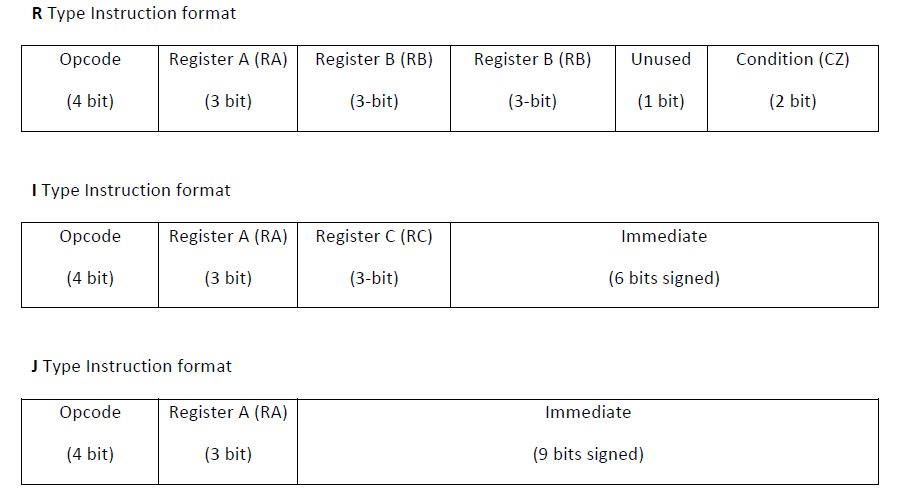
\includegraphics[width=1\textwidth]{instr_type.JPG}
    \caption{The instruction set }
    \label{fig:awesome_image}
\end{figure}


\vspace{3cm}

\begin{figure}[h]
    \centering
    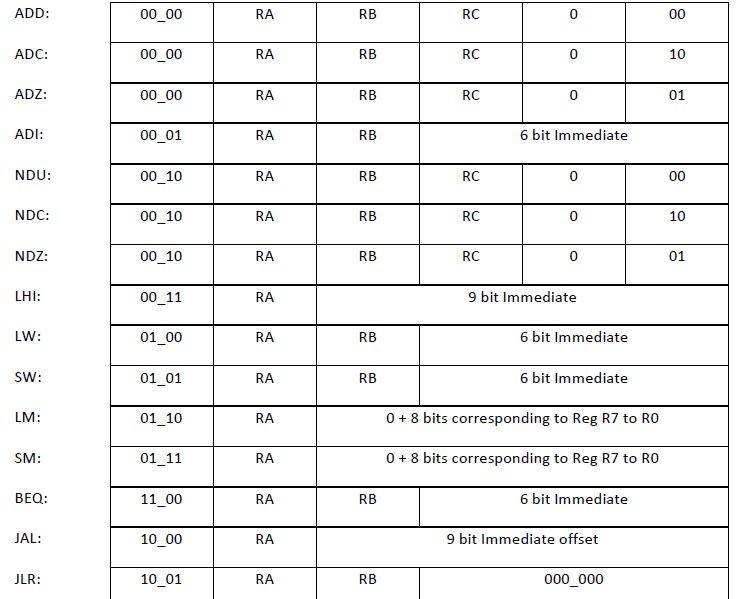
\includegraphics[width=1\textwidth]{instr_enc.JPG}
    \caption{16-bit instruction encoding }
    \label{fig:awesome_image}
\end{figure}

\hspace*{-2cm}\begin{figure}[h]
        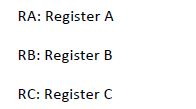
\includegraphics[width=0.3\textwidth]{reg_desrcp.JPG}
    \label{fig:awesome_image}
\end{figure}

%----------------------------------------------------------------------------------------
%	CHAPTER 3
%----------------------------------------------------------------------------------------

\chapterimage{ch_image.jpg} % Chapter heading image

\chapter{Datapath}

\section{Elements}
The datapath consists of the described units: \\ \\
\textbf{(1) Register File :} The module consists of eight 16-bit clocked registers (R0 to R7). This module has 4 inputs : 3 input addresses (add1, add2, add3) 8bit each and 1 data input (16bit). There are 2 output data sequences, corresponding to the first two input addresses, add1 and add2. Control signal Rf\_wen is involved to enable the writing to the registers.  \\ \\ \textbf{(2) ALU :} The logic unit supports two operations : ADD and NAND, to implements different instructions and for incrementing desired variables. The module is combinational in nature, meaning the desired data output would be obtained in the same cycle when the two operands are fed. Two flags CY (carry) and Z (zero) are associated with the ALU, which would be written to the CZ module defined in the datapath. A clocked register, T1, stores the computed ALU result. \\ \\ \textbf{(3) Multiplexers :} For proper instructor execution, different modules need to be enabled or disabled, along with proper routing of data to these modules. This is achieved using MUXes, having variable no. of control signals bits. These would be described later. \\ \\ \textbf{(4) CZ module :} This module is used to generate a conditional write\_enable signal to the Register File module based on previous CY and Z bits. Thus, this conditional signal would be required to implement ADZ, ADC, NDZ and NDC instruction. \\ \\ \textbf{(5) Registers :} Temporary registers A and B are used to store output results of the register file. Register T1 is similarly used to store the ALU result. \\ \\ \textbf{(6) Memory* :} This module is connected to different modules in the datapath. It has a size of 64bytes, controlled by write\_enable signal, with multiplexed input data.\\ \textbf{(7) Priority Encoder :} This module serves an essential purpose in reducing the cycles in LM and SM instructions by rendering the RF addresses corresponding to the set bits in instructions last 8 bits.
\\ \\ \textbf{(8) Sign Extenders :} This module appends zeroes at the beginning of the immediate bits, \\ Usage: extending Imm6 and Imm9 in immediate addressing
 \\ \\ \textbf{(9) Data Shifters :} This module is used  to convert a 9 bit value to 16 bit by padding zeroes at the end.\\ \\
 
 \section{Design Specifications}
Design Specifications to incorporate all corner cases (well to the best of our knowledge :)  ) are as follows :
\begin{itemize}
\item R7 is our PC and  we have PC\_enable to to update it when needed.
\item R7 = Ra + Rb is a branch instruction and in our case in any instruction the PC updation part occurs in the last states of the operation so it wouldn't affect the corner case.
\item There is a slave register CZ\_reg which takes care of this and is written to only in the ADD family of operations as mentioned in the project specifications.
As we mentioned in the lab, we have a temp\_A register to store value of A before address increment which takes care of this case.
\item We are using a priority encoder to optimize the states and cycles taken by the LM, SM instructions. Now the  cycles are equal to the number of bits set in the imm8 given in the instruction. 
\item We have extended the sign of the bits of the immediate field to ensure compatibility. 
\end{itemize}
\newpage

\section{Control Signals Interpretation} 
The different control signals to MUX's are mentioned here: \\
These multiplexers have different combination of no. of inputs and control signals, hence they are defined differently in the datapath.
\vspace{1cm}
\begin{multicols}{3}
\begin{center}
 \begin{tabular}{||c|c||} 
 \hline
 \multicolumn{2}{|c|}{Mux1\_ALU\_B (3bit)} \\
 \hline
 Mux Signal & Input \\ [0.5ex] 
 \hline\hline
 000 & 16'd0  \\ 
 \hline
 001 & 16'd01  \\
 \hline
 010 & B  \\
 \hline
 011 & imm6  \\
 \hline
 100 & addIncrement \\ [1ex] 
 \hline
\end{tabular}
\end{center}


\begin{center}
 \begin{tabular}{||c|c||} 
 \hline
 \multicolumn{2}{|c|}{Mux2\_ALU\_A (3bit)} \\
 \hline
 Mux Signal & Input \\ [0.5ex] 
 \hline\hline
 000 & 16'd0  \\ 
 \hline
 001 & 16'd01  \\
 \hline
 010 & shift7  \\
 \hline
 011 & imm6  \\
 \hline
 100 & imm9 \\
 \hline
 101 & A  \\
 \hline
 110 & tempA  \\ [1ex]
 \hline
\end{tabular}
\end{center}


\begin{center}
 \begin{tabular}{||c|c||} 
 \hline
 \multicolumn{2}{|c|}{Mux3\_RF\_wen (2bit)} \\
 \hline
 Mux Signal & Input \\ [0.5ex] 
 \hline\hline
 00 & 1'b0  \\ 
 \hline
 01 & 1'b1  \\
 \hline
 10 & CZ  \\
 \hline
 11 & addrIncrement\_out  \\ [1ex] 
 \hline
\end{tabular}
\end{center}

\end{multicols}
\vspace{0.5cm}
\begin{multicols}{3}

\begin{center}
 \begin{tabular}{||c|c||} 
 \hline
 \multicolumn{2}{|c|}{Mux\_4\_RF\_wadd (3bit)} \\
 \hline
 Mux Signal & Input \\ [0.5ex] 
 \hline\hline
 000 & regA  \\ 
 \hline
 001 & regC  \\
 \hline
 010 & lm\_sm\_addr  \\
 \hline
 011 & 3'b111  \\
 \hline
 100 & regB \\ [1ex] 
 \hline
\end{tabular}
\end{center}

\begin{center}
 \begin{tabular}{||c|c||} 
 \hline
 \multicolumn{2}{|c|}{Mux5\_RF\_read2 (2bit)} \\
 \hline
 Mux Signal & Input \\ [0.5ex] 
 \hline\hline
 00 & regB  \\ 
 \hline
 01 & lm\_sm\_addr  \\
 \hline
 10 & 3'b111  \\ [1ex] 
 \hline
\end{tabular}
\end{center}


\begin{center}
 \begin{tabular}{||c|c||} 
 \hline
 \multicolumn{2}{|c|}{Mux6\_RF\_dataIn (1bit)} \\
 \hline
 Mux Signal & Input \\ [0.5ex] 
 \hline\hline
 0 & memout  \\ 
 \hline
 1 & T1  \\ [1ex] 
 \hline
\end{tabular}
\end{center}
\end{multicols}
\vspace{0.5cm}

\begin{multicols}{3}

\begin{center}
 \begin{tabular}{||c|c||} 
 \hline
 \multicolumn{2}{|c|}{Mux8\_memwrite (2bit)} \\
 \hline
 Mux Signal & Input \\ [0.5ex] 
 \hline\hline
 00 & 1'b0  \\ 
 \hline
 01 & 1'b1  \\
 \hline
 010 & mux7  \\
 \hline
 11 & imm6  \\ [1ex] 
 \hline
\end{tabular}
\end{center}

\begin{center}
 \begin{tabular}{||c|c||} 
 \hline
 \multicolumn{2}{|c|}{Mux9\_memDataIn (1bit)} \\
 \hline
 Mux Signal & Input \\ [0.5ex] 
 \hline\hline
 0 & A  \\ 
 \hline
 1 & B  \\ [1ex] 
 \hline
\end{tabular}
\end{center}
\end{multicols}
%\begin{figure}[h]
%    \centering
%    \includegraphics[width=6.9cm, height=16cm]{mux_signals.jpg}
%    \caption{Control signals to MUXes }
%    \label{fig:awesome_image}
%\end{figure}
%----------------------------------------------------------------------------------------
%	CHAPTER 4
%----------------------------------------------------------------------------------------
\vspace{2cm}
\section{Datapath}
\vspace*{-1cm}
\begin{figure}[h]
    \centering
    High Resolution SVG version of the datapath diagram can be found at : \\ \url{https://www.ee.iitb.ac.in/student/\~meetshah1995/files/datapath.svg}
    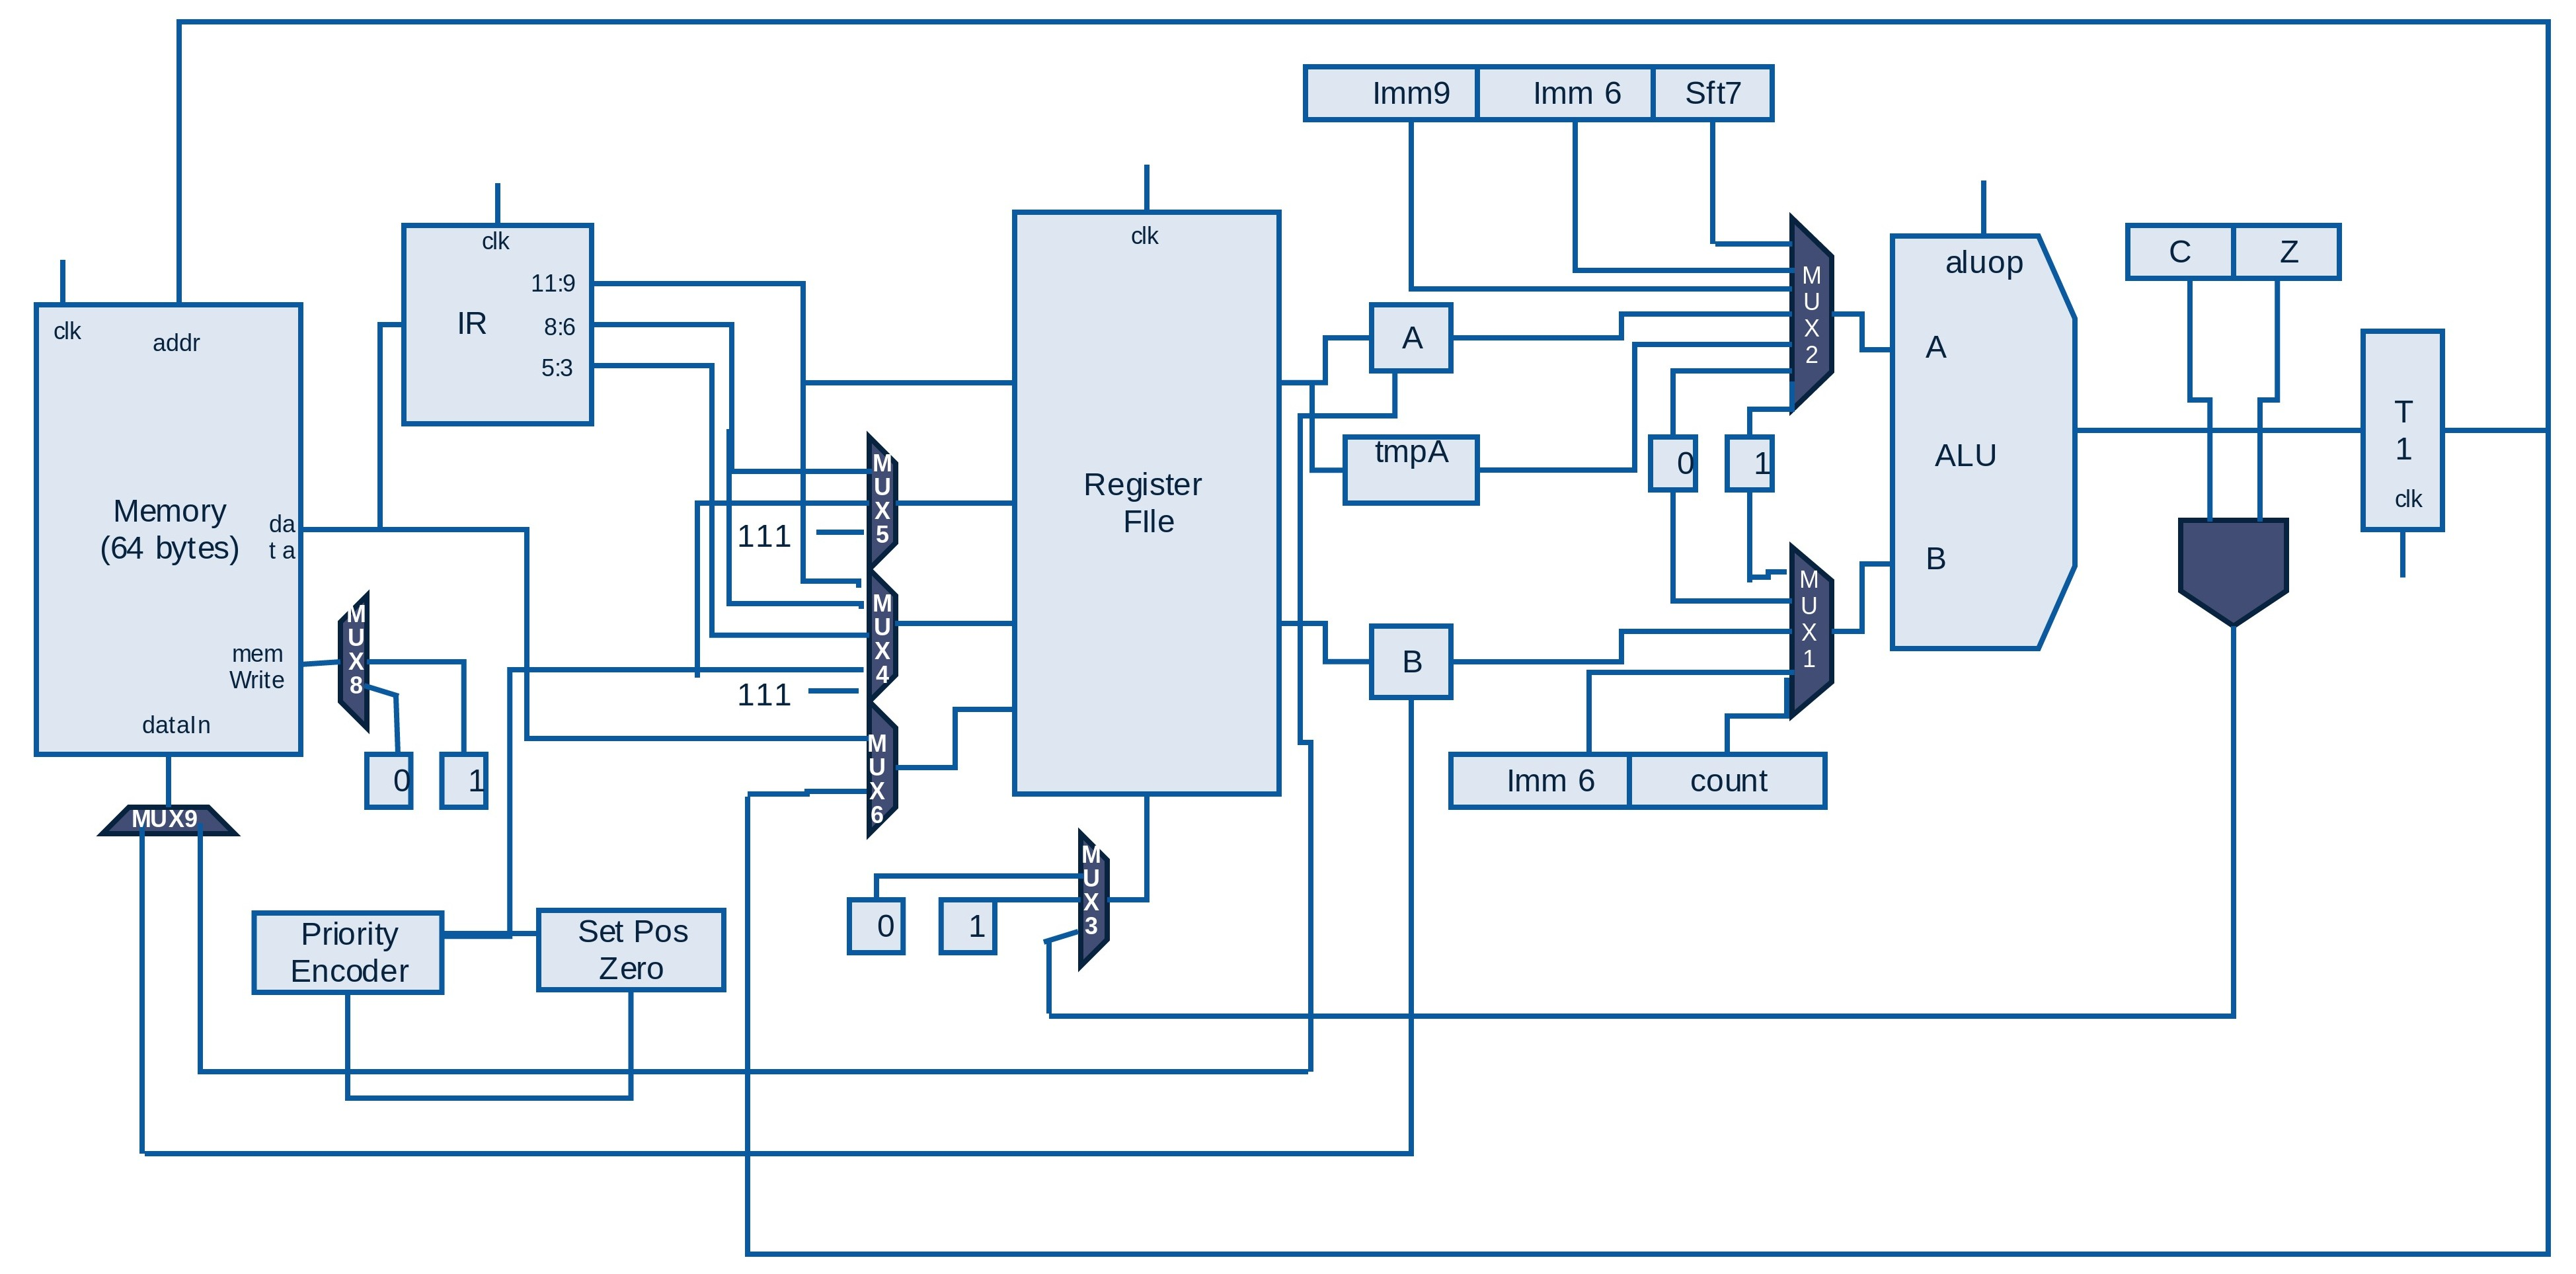
\includegraphics[scale=0.13,angle=90]{iitb_risc_15.jpg}
    \caption{Proposed Datapath }
    \label{fig:awesome_image}
\end{figure}
\newpage

\chapterimage{ch_image.jpg}

\chapter{Controller}


\section{State Description}
Writeup for different states involved for each instruction(These are shown sequentially going from left to right):\\ \\

\textbf{1. ADD }
\begin{center}
 \begin{tabular}{ | m{5em} | m{5em} | m{5em} | m{5em} | m{7em} | } 
 \hline
 0 & 1 & 2 & 3 & 4 \\ [0.5ex] 
 \hline
 Instruction gets stored in IR & Values of reg read into A and B for Add & Added answer written into Rc & Read PC into B and +1 passed to ALU & PC+1 stored in T1; ready to write that in PC (will be updated automatically in next cycle) \\ [1ex]
 \hline
\end{tabular}
\end{center}

\vspace{0.5cm}

\textbf{2. ADC }
\begin{center}
 \begin{tabular}{ | m{5em} | m{5em} | m{5em} | m{7em} | m{7em} | m{7em} | } 
 \hline
 0 & 1 & 5 & 7 & 3 & 4 \\ [0.5ex]
 \hline
 Instruction gets stored in IR & Values of reg read into A and B for Add & Logical combination of the carry and zero bits is stored in CZ\_reg for Add & Depending upon logical combination of the carry and zero bits added value is written in Rc & Read PC into B and +1 passed to ALU & PC+1 stored in T1; ready to write that in PC (will be updated automatically in next cycle)  \\ [1ex]
 \hline
\end{tabular}
\end{center}

\newpage 

\textbf{3. ADZ }
\begin{center}
 \begin{tabular}{ | m{5em} | m{5em} | m{5em} | m{5em} | m{7em} | m{7em} | } 
 \hline
 0 & 1 & 5 & 7 & 3 & 4 \\ [0.5ex]
 \hline
 Instruction gets stored in IR & Values of reg read into A and B for Add & Logical combination of the carry and zero bits is stored in CZ\_reg for Add & Depending upon logical combination of the carry and zero bits added value is written in Rc & Read PC into B and +1 passed to ALU & PC+1 stored in T1; ready to write that in PC (will be updated automatically in next cycle)  \\ [1ex]
 \hline
\end{tabular}
\end{center}

\vspace{1cm}

\textbf{4. NDU }
\begin{center}
 \begin{tabular}{ | m{5em} | m{5em} | m{5em} | m{7em} | m{7em} | } 
 \hline
 0 & 8 & 9 & 3 & 4 \\ [0.5ex]
 \hline
 Instruction gets stored in IR & Values of reg read into A and B for NAND & NANDed answer written into Rc & Read PC into B and +1 passed to ALU & PC+1 stored in T1; ready to write that in PC (will be updated automatically in next cycle)  \\ [1ex]
 \hline
\end{tabular}
\end{center}

\vspace{1cm}

\textbf{5. NDC }
\begin{center}
 \begin{tabular}{ | m{5em} | m{5em} | m{5em} | m{7em} | m{5em} | m{7em} | } 
 \hline
 0 & 8 & 10 & 7 & 3 & 4 \\ [0.5ex]
 \hline
 Instruction gets stored in IR & Values of reg read into A and B for NAND & Logical combination of the carry and zero bits is stored in CZ\_reg for NAND & Depending upon logical combination of the carry and zero bits added value is written in Rc & Read PC into B and +1 passed to ALU & PC+1 stored in T1; ready to write that in PC (will be updated automatically in next cycle)  \\ [1ex]
 \hline
\end{tabular}
\end{center}



\textbf{6. NDZ }
\begin{center}
 \begin{tabular}{ | m{5em} | m{5em} | m{5em} | m{7em} | m{5em} | m{7em} | } 
 \hline
 0 & 8 & 10 & 7 & 3 & 4 \\ [0.5ex]
 \hline
 Instruction gets stored in IR & Values of reg read into A and B for NAND & Logical combination of the carry and zero bits is stored in CZ\_reg for NAND & Depending upon logical combination of the carry and zero bits added value is written in Rc & Read PC into B and +1 passed to ALU & PC+1 stored in T1; ready to write that in PC (will be updated automatically in next cycle)  \\ [1ex]
 \hline
\end{tabular}
\end{center}

\vspace{0.5cm}

\textbf{7. ADI }
\begin{center}
 \begin{tabular}{ | m{5em} | m{5em} | m{7em} | m{5em} | m{8em} | } 
 \hline
 0 & 11 & 12 & 3 & 4 \\ [0.5ex]
 \hline
 Instruction gets stored in IR & Pass Imm6 to input B of ALU to be added in the next state & Added answer written into Rb & Read PC into B and +1 passed to ALU & PC+1 stored in T1; ready to write that in PC (will be updated automatically in next cycle)\\ [1ex]
 \hline
\end{tabular}
\end{center}

\vspace{0.5cm}

\textbf{8. LHI }
\begin{center}
 \begin{tabular}{ | m{5em} | m{5em} | m{7em} | m{5em} | m{8em} | } 
 \hline
 0 & 20 & 21 & 3 & 4 \\ [0.5ex]
 \hline
 Instruction gets stored in IR & Pass Shifted 7 Value and 0 to ALU for loading & Loaded Value Returned to Ra & Read PC into B and +1 passed to ALU & PC+1 stored in T1; ready to write that in PC (will be updated automatically in next cycle)\\ [1ex]
 \hline
\end{tabular}
\end{center}

\vspace{1cm}

\textbf{9. SW }
\begin{center}
 \begin{tabular}{ | m{5em} | m{5em} | m{7em} | m{5em} | m{5em} | m{7em} | } 
 \hline
 0 & 15 & 16 & 17 & 3 & 4 \\ [0.5ex]
 \hline
 Instruction gets stored in IR & Imm 6 and reg B is passed to ALU & Resultant memory address, is passed to memory block & Desired data is written in the memory & Read PC into B and +1 passed to ALU & PC+1 stored in T1; ready to write that in PC (will be updated automatically in next cycle)\\ [1ex]
 \hline
\end{tabular}
\end{center}

\newpage

\textbf{10. LW }
\begin{center}
 \begin{tabular}{ | m{5em} | m{7em} | m{5em} | m{5em} | m{7em} | } 
 \hline
 0 & 15 & 18 & 3 & 4 \\ [0.5ex]
 \hline
 Instruction gets stored in IR & Imm 6 and reg B is passed to ALU & Data output from memory is stored in the Register File & Read PC into B and +1 passed to ALU & PC+1 stored in T1; ready to write that in PC (will be updated automatically in next cycle)\\ [1ex]
 \hline
\end{tabular}
\end{center}

\vspace{0.5cm}

\textbf{11. BEQ }
\begin{center}
 \begin{tabular}{ | m{5em} | m{5em} | m{5em} | m{5em} | m{5em} |  m{7em} |} 
 \hline
 0 & 22 & 23 & 24 (if compare high) & 3 (else) & 4 \\ [0.5ex]
 \hline
 Instruction gets stored in IR & reg A and reg B values are loaded & Same as previous state to ensure proper data storage in T1 register & Imm 6 and reg B is passed to ALU & Read PC into B and +1 passed to ALU & PC+1 stored in T1; ready to write that in PC (will be updated automatically in next cycle)\\ [1ex]
 \hline
\end{tabular}
\end{center}


\textbf{12. JAL }
\begin{center}
 \begin{tabular}{ | m{5em} | m{5em} | m{5em} | m{5em} | m{5em} |  m{7em} |} 
 \hline
 0 & 3 & 25 & 26 & 27 & 4 \\ [0.5ex]
 \hline
 Instruction gets stored in IR & Read PC into B and +1 passed to ALU & Store PC+1 in reg A & add imm6 with PC, caring not to set the carry & Store the obtained result in PC & PC+1 stored in T1; ready to write that in PC (will be updated automatically in next cycle)\\ [1ex]
 \hline
\end{tabular}
\end{center}
 
\vspace{0.5cm}

\textbf{13. JLR }
\begin{center}
 \begin{tabular}{ | m{5em} | m{5em} | m{5em} | m{5em} | m{5em} |  m{7em} |} 
 \hline
 0 & 3 & 25 & 28 & 29 & 4 \\ [0.5ex]
 \hline
 Instruction gets stored in IR & Read PC into B and +1 passed to ALU & Store PC+1 in reg A & Pass reg B and 0 to ALU & Store obtained result in PC & PC+1 stored in T1; ready to write that in PC (will be updated automatically in next cycle)\\ [1ex]
 \hline
\end{tabular}
\end{center}

\vspace{0.5cm}

\newpage 
\textbf{14. LM }
\begin{center}
 \begin{tabular}{ | m{5em} | m{5em} | m{5em} | m{5em} | m{5em} | m{5em} |  m{7em} |} 
 \hline
 0 & 30 & 31 & 32 & 33 (Decide Repeat) & 3 & 4 \\ [0.5ex]
 \hline
 Instruction gets stored in IR & Set the Mux4 to take address from the priority encoder and enable the Priority encoder & Enable data writing for RF & Disable write for Atmp & Values written into RF, disable wRF, T1write and increment counter & Read PC into B and +1 passed to ALU  & PC+1 stored in T1; ready to write that in PC (will be updated automatically in next cycle)\\ [1ex] 
 \hline
\end{tabular}
\end{center}

\vspace{0.5cm}

\textbf{15. SM }
\begin{center}
 \begin{tabular}{ | m{5em} | m{5em} | m{5em} | m{5em} | m{7em} | m{5em} |  m{7em} |} 
 \hline
 0 & 34 & 35 & 36 & 37 (Decide Repeat) & 3 & 4 \\ [0.5ex]
 \hline
 Instruction gets stored in IR & Set the Mux5 to take input from the priority encoder address and enable the Priority encoder & Enable the memory\_write signal in the controller & Wait for the memOut to Load into the corresponding memory address & Disable the memory\_write, disable the priority encoder and increment the counter  & Read PC into B and +1 passed to ALU  & PC+1 stored in T1; ready to write that in PC (will be updated automatically in next cycle)\\ [1ex] 
 \hline
\end{tabular}
\end{center}

\newpage

\section{Finite State Machine}

\begin{figure}[h]
    \centering
    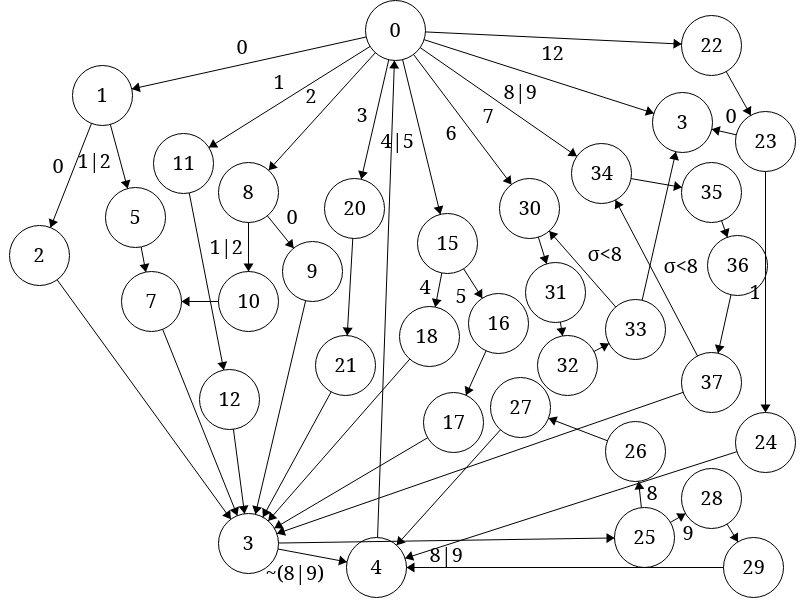
\includegraphics[width=14.5cm,height=15.6cm]{FSM.png}
    \caption{The State Transition flow }
    \label{fig:awesome_image}
\end{figure}
\newpage


%----------------------------------------------------------------------------------------
%	CHAPTER 5
%----------------------------------------------------------------------------------------
\chapterimage{ch_image.jpg}

\chapter{Testing}

\section{Test Cases}
\vspace{1cm}
Default register values : \\
reg0        16'b0000000000000011    \\
reg1     	16'b1111111111111111	\\
reg3    	16'b0000000000000001	\\

\textsc{Test 1:} \\
\textit{
mem[0] <= 16'b0000001011110000; \textcolor{blue}{// ADD  R1  R3  R6} \\
mem[1] <= 16'b0010001011101000; \textcolor{blue}{// NDU  R1  R3  R5} \\
mem[2] <= 16'b0000001011100010;	\textcolor{blue}{// ADC  R1  R3  R4} \\
mem[3] <= 16'b0010001011010001;	\textcolor{blue}{// NDZ  R1  R3  R2} \\
mem[4] <= 16'b0001001011110000;	\textcolor{blue}{// ADI  R3  R1  6'b110000} \\
}

\vspace{1cm}

\textsc{Test 2:} \\
\textit{
mem[0] <= 16'b1100001011000010; \textcolor{blue}{// BEQ  R1  R3  6'b000010} \\
mem[1] <= 16'b0011001101101001;  \textcolor{blue}{// LHI  R1  9'b101101001} \\
mem[2] <= 16'b0101001011000011;	\textcolor{blue}{// SW  R1  R3  6'b000011} \\
mem[3] <= 16'b0100010011000011;	\textcolor{blue}{// LW  R2  R3  6'b000011} \\
}

\vspace{1cm}

\textsc{Test 3:} \\
\textit{
mem[0] <= 16'b1000000000000011; \textcolor{blue}{// JAL  R0  9'b000000011} \\
mem[1] <= 16'b0000001011100010; \textcolor{blue}{// ADC  R1  R3  R4} \\
mem[2] <= 16'b0010001011101000;	\textcolor{blue}{// NDU  R1  R3  R5} \\
mem[3] <= 16'b0010001011010001;	\textcolor{blue}{// NDZ  R1  R3  R2} \\
mem[4] <= 16'b0001001011110000;	\textcolor{blue}{// ADI  R3  R1  6'b110000} \\
}

\vspace{1cm}

\textsc{Test 4:} \\
\textit{
mem[0] <= 16'b1001000010000000; \textcolor{blue}{// JLR  R0  R2 } \\
mem[1] <= 16'b0000001011100010; \textcolor{blue}{// ADC  R1  R3  R4} \\
mem[2] <= 16'b0010001011101000;	\textcolor{blue}{// NDU  R1  R3  R5} \\
}

\vspace{1cm}

\textsc{Test 5:} \\
\textit{
mem[0] <= 16'b0110000001100100; \textcolor{blue}{// LM   R0  9'b001100100} \\
mem[1] <= 16'b0000001011100000; \textcolor{blue}{// ADD  R1  R3  R4} \\
mem[2] <= 16'd1; \\
mem[3] <= 16'd2; \\
mem[4] <= 16'd3; \\
mem[5] <= 16'd4; \\
mem[6] <= 16'd5; \\
mem[7] <= 16'd6; \\
mem[8] <= 16'd7; \\
mem[9] <= 16'd8; \\
}

\vspace{1cm}

\textsc{Test 6:} \\
\textit{
mem[0] <= 16'b0111000001100100; \textcolor{blue}{// SM  R0  9'b001100100} \\
mem[1] <= 16'b0000001011100000; \textcolor{blue}{// ADD  R1  R3  R4} \\
}


\end{document}